% TODO: Include command for "buzzwords" or "keywords", instead of just bolding them.

\documentclass[fontsize=12pt,twoside=on,openright,parskip=half]{scrbook}
\usepackage[T1]{fontenc}
\usepackage{lmodern}
\usepackage{listings}
\usepackage{xcolor}
\usepackage{graphicx}
\usepackage[english]{babel}
\usepackage{blindtext}
\usepackage{hyperref}
\definecolor{skyblue}{RGB}{189,227,255}
\definecolor{cornflower}{RGB}{51,153,255}
\newcommand{\code}[1]{\colorbox{skyblue}{\texttt{#1}}}
\renewcommand*\familydefault{\sfdefault}
\setkomafont{disposition}{\color{cornflower}\bfseries}
\graphicspath{ {./images/} }

\title{The CS Napkin}
\subtitle{A compilation of thoughts, notes, and ideas from my undergrad education}
\author{Pranavi Reddi \& Arim Lim}
\date{21 Nov 2023\thanks{First drafted on 19 Nov 2023}}

\begin{document}

\maketitle

\tableofcontents

\chapter{Foreword}

If you’re reading this, you’re most likely planning to pursue the CS major at
Duke University. You’ve probably taken either 101 or 201 (or both), and are
wondering where to go next. The start of the Duke CS major is pretty
cut-and-dry: you take 201, then one of 250/210 (the introductory systems
courses) and 230 (Discrete Math). Eventually, you’ll take 330. Pretty
straightforward, right? But what comes after? What comes in-between?

Beyond its core classes, the CS major has plenty of room to explore, but its
flexibility sometimes gives rise to a good deal of confusion about
dependencies. When should I take X class? Do I know enough to take Y class? And
why should I even take Z class at all?

We hope that our CS “Napkin” will help answer some of these questions for you.
It provides an overview of the content of each class; each section is a bit
more detailed than a syllabus with (hopefully) helpful tips sprinkled
throughout. Not only do we provide summaries of the class, we also start each
section with a short meta-commentary that explains where each class slots into
the big picture of a bachelor’s in CS, and why you might want to take said
class in the first place.

We were heavily inspired by \href{https://web.evanchen.cc/napkin.html}{Evan
Chen’s napkin} about college-level math, and we highly recommend checking it
out.

\chapter{Prerequisites}

We expect readers of the Napkin to have programmed before, on the scale of
anything including but not limited to:

\begin{itemize}
	\item that CS50 online course offered by Harvard
	\item any CS101 college course
	\item AP CS Principles… something along those lines?
\end{itemize}

We expect you to have understood and used basic programming concepts such as:
for/while loops, conditional control flow, variables, and functions. 

The Napkin is programming-language-agnostic, though we do mention
course-specific languages and their details (Java, C, etc). But in the wise
words of software developer Tsoding, we strongly believe that:

\begin{figure}[h]
\centering
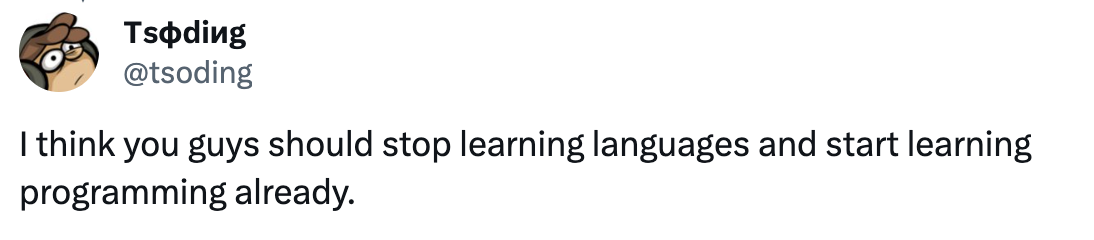
\includegraphics[scale=0.8]{tsoding}
\end{figure}

\chapter{The Missing Semester}

Who’da thunk it? The geniuses at MIT have pioneered what we think is a
fantastic idea: the missing semester for CS majors. Their rationale
(\textbf{emphasis} ours):
\begin{quote}

	Classes teach you all about advanced topics within CS, from operating
	systems to machine learning, but there’s one critical subject that’s rarely
	covered, and is instead left to students to figure out on their own:
	\textbf{proficiency with their tools}. We’ll teach you how to master the
	command-line, use a powerful text editor, use fancy features of version
	control systems, and much more!

\end{quote} They run the gamut of practical skills, most if not all of which we
believe are invaluable tools for a computer scientist in almost any context.
These skills aren’t covered in any significant depth at Duke either! We’ll
briefly go over some of them in the Napkin, but we highly suggest checking out
the \href{https://missing.csail.mit.edu/}{original MIT website}.

\begin{itemize}
	\item Version control/Git crash course
	\item Basic terminal commands
	\item Unit testing
\end{itemize}

\section*{Version Control \& Git}

Git was created by the same guy that was behind the first Linux kernel:
computer programmer Linus Torvalds. It is a powerful piece of software that
allows for non-linear development across multiple branches, across multiple
machines. In other words, a \textbf{distributed version control system}. 

\blindtext

\section*{Intro to the terminal \& shell scripting}

What is the terminal? aka the shell, aka the command line? These terms are all
used interchangeably, and they all mean pretty much the same thing. Let’s go
through a brief history of the terminal: once upon a time, terminals were the
only way to interact with computers. \textbf{UNIX}, a very important operating
system, was written in such an era\footnote{If you want to learn more, I highly
recommend \textit{The Unix Programming Environment} by Brian Kernighan, which
is slightly outdated but serves both as a delightful artifact of CS history and
a helpful introduction to the Unix command line (and also C programs!).}. There
were no graphical user interfaces (GUIs), much less a notion of a desktop with
icons for apps and folders.

\begin{figure}[h]
\centering
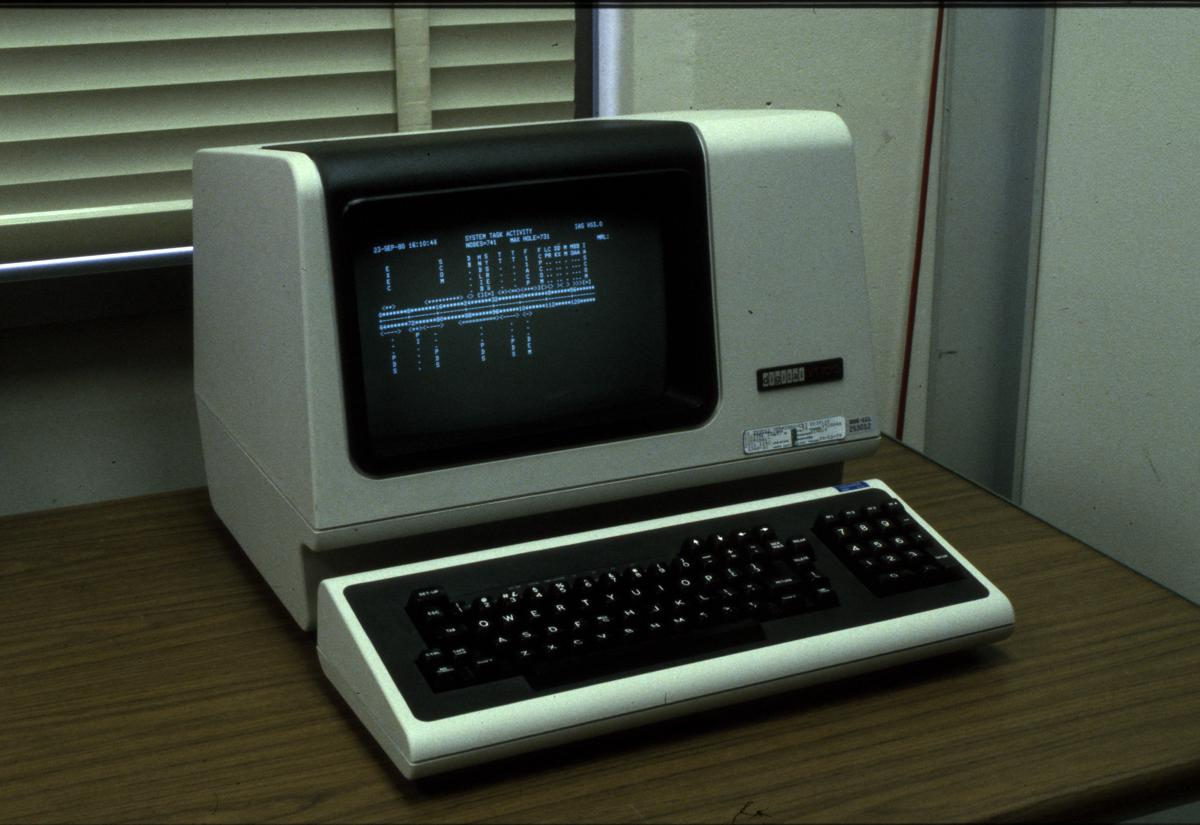
\includegraphics[scale=0.2]{dec}
\caption{\small{The DEC VT102 terminal, with a CRT monitor. It was common for monitors
to be 80 characters wide, a convention that still carries over today for many
programmers’ coding style guidelines (e.g.\ in the Linux kernel)}}
\end{figure}

They were and \emph{still are} powerful ways to interact with computers! In
many use-cases, the terminal is much more efficient than the click-drag-drop
interface of a GUI, and hell of a lot more configurable. Though it may seem
intimidating at first, once you get comfortable with a handful of commands,
popping open the terminal will soon feel more like a superpower than fumbling
with a black box.

All of the commands we mention here will be applicable to both MacOS and Linux
(oh, the joy of working on UNIX-likes!). We assume that your shell is either
\textbf{bash} (the default on most Linux distributions) or \textbf{zsh} (the
default on MacOS). If you aren’t sure, you can always type \code{echo \$0} into
the command line and press enter; the terminal should tell you what shell
you’re using. 

Before we start for real, a quick word about \code{man pages}. These are
basically documentation files that are stored on any UNIX-based system. The
Linux man pages specifically are available online, and you can also download
them from this git repo. MacOS also has its own man pages.

You can access any man page of any C standard library function, or shell
command simply by entering \code{man function-name} in the terminal, i.e.,
\code{man printf} or \code{man grep}. It is an invaluable tool for any systems
programmer. Although they may be hard to read at first, eventually it becomes
second nature, and they are infinitely better than those janky w3schools pages
(which are misleading and often contain genuinely dangerous snippets of C
code). If you forget how to use a certain shell command (this occurs often,
especially with the countless flags associated with something even as simple as
\code{ls}!) the man pages will always be there for you. And what’s more
heartwarming than that?

\code{\$ echo blah} \\*
\textbf{Outputs whatever you put in as an argument}. The argument could be a
variable, such as in the example of \code{echo \$0} previously shown. Try
entering “echo hello world” into your prompt (represented here as a dollar
sign). There, you’ve written your first shell script, yay!

\code{\$ cat file-name1 file-name2 \ldots} \\*
\textbf{Outputs the contents of a file}. Its name is short for “concatenate”,
and no surprise, its canonical use is to concatenate different files together
into one stream.

\code{\$ ls path-to-directory (optional)} \\*
\textbf{Lists the contents of whatever directory you’re currently in}. Common
and useful tags (flags that you can append to the original command to get a
more detailed output) include -a, which lists even hidden files (files whose
names start with “.”, these are usually configuration files for various
applications), -l, which includes information about size, ownership,
permissions, etc.\ e.g., ls -al is a very commonly used command.

\code{\$ cd path-to-directory (optional)} \\*
\textbf{Changes the directory you’re in}. If you don’t supply an argument, cd
will take you back to your home directory. Take care to note when you’re in
your root directory (\code{/}) versus your home (\code{\~/}), because they can
seem quite similar though they are radically different places in your file
system.

\code{\$ mkdir directory-name} \\*
\textbf{Creates a directory}.

\code{\$ touch file-name1 file-name2 \ldots} \\*
\textbf{Creates (a) file(s)}.

\code{\$ rm file-name1 file-name2 \ldots} \\*
\textbf{Removes (a) file(s)}. Unlike putting your files in the trash can, when
you rm a file, it is gone forever, so be very careful. You can be more careful
by adding \code{-i} (interactive) to the command; the shell will prompt you for
permission before it deletes anything. You can remove directories by adding
\code{-r} (recursive) to the command, and you can be very uncareful by adding
\code{-f} (force) to the command; the shell will NOT prompt you for permission
before it deletes.\ \code{rm -rf} for deleting a directory is a very common
command, but wield it with caution!

\code{\$ mv old-path-name new-path-name} \\*
\textbf{Renames/moves a file or directory}. The way the UNIX file system is set
up, moving files/directories and renaming their paths are technically the same
thing

\code{\$ cp old-path-name new-path-name} \\*
\textbf{Copies original file to a new file}. Very useful for quickly making
backup files.

\code{\$ diff file-name1 file-name2} \\*
\textbf{Returns all the different lines between two files}. Yes, this is
similar to git diff!

\code{\$ grep ``string or regular expression'' file-name1} \\*
\textbf{Searches for and prints a regular expression}\footnote{Regular
	expressions (aka ``regexes''), invented by computer scientist Stephen
	Kleene (who also invented recursion theory, among other things), are one of
	those concepts where if you put in a couple hours upfront to learn their
	basics, it will pay itself off many times over in the future.
\href{https://regexone.com/} is a fantastic website for getting started. }.
Grep stands for ``\textbf{g}et \textbf{r}egular \textbf{e}xpression and
\textbf{p}rint'', and you can think of it as a powerful, extendable search
tool. There’s no way we can cover the world of regular expressions in this
section, but they are incredibly useful to know. For now, though, just know
that we can supply just a string as an argument and grep will print out
instances of that string in the file(s) you specify.

\code{\$ head -number file-name} \\*
\textbf{Outputs however many lines you specify from the start of the file}.

\code{\$ tail -number file-name} \\*
\textbf{Outputs however many lines you specify from the end of the file}.

Now that you know the building blocks, we are now able to see where the real
magic happens. When computer scientists were building UNIX, they also pioneered
what is known as the “\textbf{UNIX philosophy}”. Simply put, the UNIX
philosophy encourages writing simple, modular programs that can be linked
together in creative and powerful ways, just by redirecting input/output,
either using \code{``>''}, \code{``<''} or \code{``|''} (the latter symbol is
called a “pipe”, and it’s ubiquitous in shell scripts). Watch Brian Kernighan
himself demonstrate the UNIX philosophy in
\href{https://www.youtube.com/watch?v=tc4ROCJYbm0}{this video}, which I truly
believe is one of the best on YouTube. His explanation begins 6 minutes in.

\begin{figure}[h]
\centering
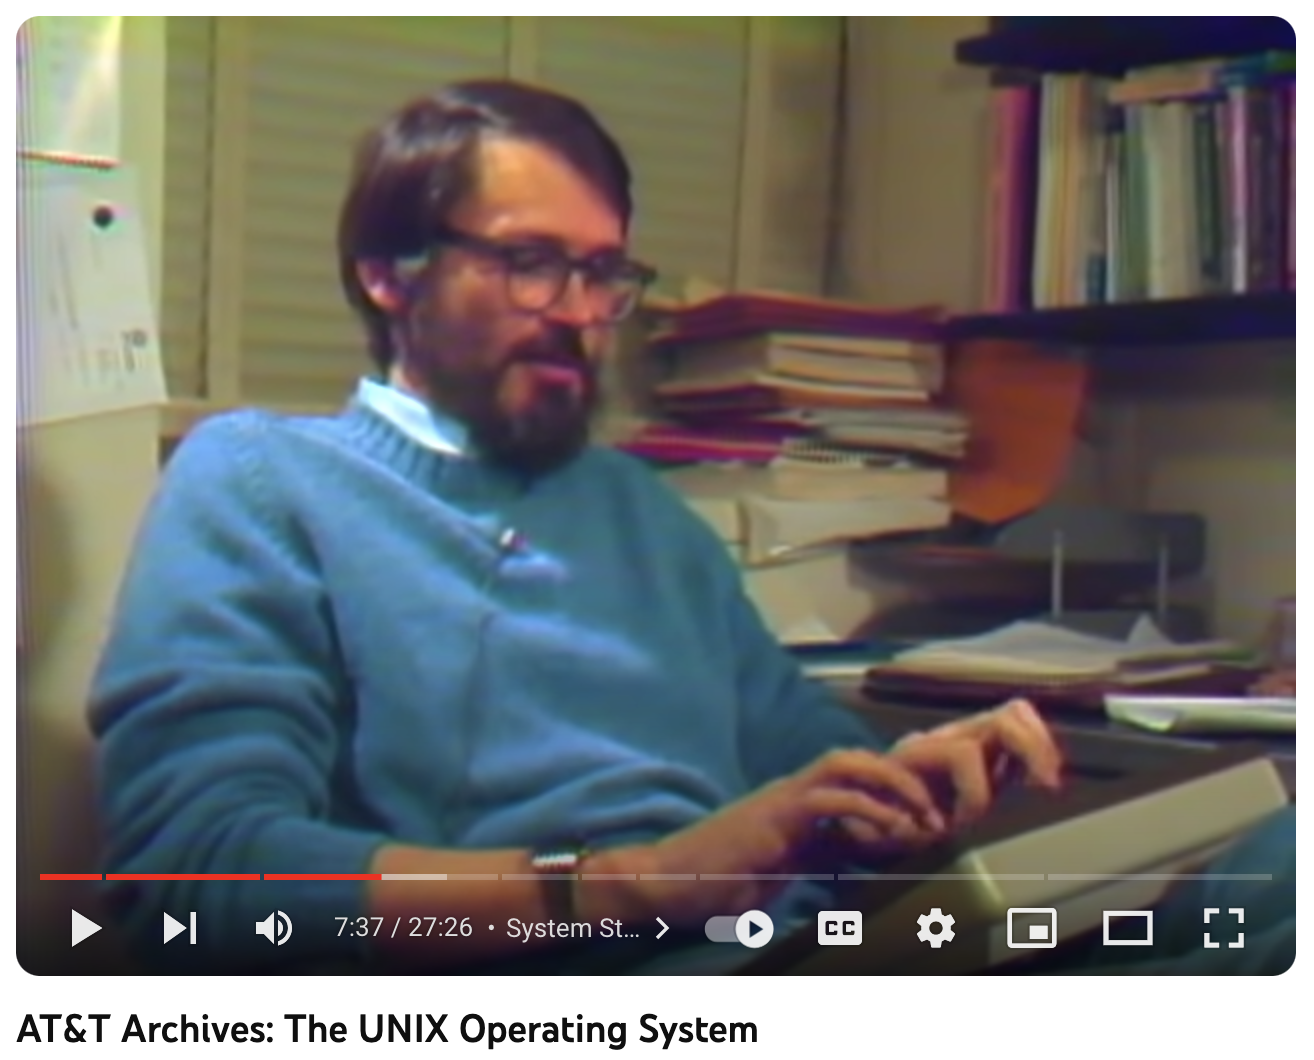
\includegraphics[scale=0.5]{unixprogrammer}
\end{figure}

Once you understand how his command line dictionary program works with pipes,
you will pretty much be set for life (well, set for a computer science degree).
Shell scripting is a relatively obscure art, and its syntax can often feel
unintuitive (there are quite a few pitfalls depending on the shell you’re
using), but its interactive nature makes it very entertaining to tinker with.
If you want to move forward and write more substantial scripts, try installing
\textbf{shellcheck}, which is what it sounds like: a neat static code analysis
tool just for shell scripts.

Standalone shell script files (often ending with \code{.sh}) require something
called a ``\textbf{shebang}'' at the top of a file. It looks something like
\code{\#!/usr/bin/bash}. Basically, a \code{\#!} followed by a path to your
shell. It lets the computer know which shell you want to use to run this
script. Without a shebang, the script will not run.

\section*{Unit testing}

\blindtext

\chapter{Discrete Math for Computer Science}

\section*{About this class}

CS230 is a curious class because it is generally bifurcated, depending on
whether you take it in the Spring or the Fall, and depending on the instructor
that is tasked with teaching it. Professors Carlos Tomasi and Kamesh Munagala
provide a much more conventional course that serves as a solid introduction to
theoretical computer science, with a lot of math and some Python programming
assignments. Professor Bruce Donald (who is on sabbatical at the time of
writing) teaches a much more quirky flavor of discrete math because his course
also doubles as an intro course to Scheme, a dialect of Lisp (which is a
powerful and extendable functional programming language, with much less of an
emphasis on mathematics. Also, one of the only classes on functional
programming offered at Duke!). 

In Fall ‘23, when we took the course, it was taught by Professor Kate O’Hanlon,
who taught it in the style of Professors Tomasi and Munagala (minus the
programming element— there was literally not a single line of code to be
written in the class). It’s likely that this is the vein that CS230 will
continue to be taught in.

In Spring ‘24 semester, a new course crosslisted with the Math department was
announced: CS232, which is what it sounds like: a more math-oriented flavor of
CS230 that goes in-depth into Markov Chains. If you’re a Math major or minor,
it might be better to take CS232 or even just opt for the Math substitution.

\section*{Why Discrete Math?}

As you continue to progress through your undergraduate education in computer
science, it becomes increasingly clear that the entire world of computing is
built upon a firm foundation of mathematics. Gaining a basic overview of some
of the most important concepts in the will prove to be quite valuable,
especially as you encounter more challenging topics within the field of
computing, including algorithmic design and computational theory. This section
of the napkin will serve to provide a concise introduction to the key concepts
of this course. 

\section*{Structure}

The structure of this section of the napkin will be adapted from the discrete
mathematics curriculum at Duke University. We will begin by exploring basic
logical and proof writing before moving into some more concepts related to
probability and counting and will finally end with connecting these ideas to
data structures and computer science at large.

\section*{Logic}

\subsection*{Why Logic?}

Logic enables us to clearly express ideas and arguments in ways that are free
from the confusions and generalizations of English and language in general.

\subsection*{Definitions}

\begin{itemize}
	\item Proposition:  A statement that can have a truth value (true/false)
		assigned to it.
		\begin{itemize}
			\item Ex: Ella is a robot.
			\item It is important to note that propositional logic does not
				enable us to convey relationship between distinct objects. We
				use predicate logic for this instead.
		\end{itemize}
	\item Terms:  Basic objects that can be used in a proposition or statement.
		\begin{itemize}
			\item Ex: Ella.
		\end{itemize}
	\item Variables: Placeholders for objects.
		\begin{itemize}
			\item Ex: X, Y
		\end{itemize}
	\item Predicate: Propositions with variables. They do not inherently hold a
		truth value, but can take on such a value in two cases. 
		\begin{itemize}
			\item The variables are replaced with terms.
				\begin{itemize}
					\item Ex: X is a robot. (See, this does not have a truth
						value; however, \emph{Ella} is a robot does!)
				\end{itemize}
			\item All variables are quantified.
		\end{itemize}
	\item Formula: Compound predicate
\end{itemize}

\chapter{Intro to Computer Systems}

\section*{About this class}

First, some background. CS210 is a relatively “young” class. It was first
offered in Fall 2021 as an alternative to the introductory systems course
requirement (before, all CS students had to take CS250, Computer Architecture).
It’s juggled around by various systems faculty (except for the one time that
Professor Fain co-taught it). Where CS250 focuses more on hardware and
processor design, CS210 deals with big ideas in systems from a software
programmer’s point of view. 

There’s pros and cons to 210’s newness. A pro is that its syllabus is
relatively flexible compared with 250, so the course structure is more open and
malleable to student feedback throughout the semester. A con is that there
aren’t as many resources (such as past exams and answer keys) to study from,
and indeed the syllabus varies more from instructor to instructor than 250
does, so what you get might differ a bit from what we have laid out here. For
context, we took 210 in Spring ‘22 when it was co-taught by Professors Jeff
Chase and Matthew Lentz.

Both classes have significant overlap with regards to:

\begin{itemize}
	\item C programming
	\item Binary representation of data
	\item Assembly language (notably, you are expected to produce MIPS assembly
		code in 250; you are not expected to write assembly for 210)
	\item Processes
	\item Caching
	\item Virtual memory
\end{itemize}

250 notably lacks content about the C toolchain (make files, linking, loading,
etc) and lacks more detailed discussions about concurrency (mutexes, condition
variables, the producer-consumer paradigm). 210 notably lacks content about
logic gates, processors (pipelining, for one), coding in assembly, and lacks
more detailed discussion on caching (e.g.\ cache coherence).

A major pro of taking 210 (when it is taught by either Professors Danyang Zhuo
(as it will be in Spring ‘24!) or Matthew Lentz) is that it sets you up pretty
perfectly for the other class that they share teaching responsibilities over:
310, or Introduction to Operating Systems. I recommend trying to take 210 and
310 in consecutive years or better yet, semesters—though this requires some
amount of planning, as 310 is currently not offered every semester. However,
310 (or its grad equivalent, 510) is guaranteed to be offered at least once per
year.

If you are planning to do an ECE major or minor, you must take CS250. If you’re
not, then by all means, come along for the 210 ride! 

\section*{History of UNIX, C and systems programming}

When you first learn about the history of computer systems, you realize that
most of the field’s brightest breakthroughs started off as the brainchildren of
researchers at a privately-owned laboratory called Bell Labs (yes, named after
Alexander Graham Bell!). Among these wizards were Brian Kernighan, Ken
Thompson, and Dennis Ritchie, two of whom you might recognize as the authors of
one of the most iconic CS textbooks of all time: \textbf{The C Programming
Language}, often referred to as “K\&R” (after Kernighan and Ritchie’s initials).

The C language and \textbf{UNIX} are very much intertwined, and form the basis
of many computer systems. UNIX is one of the most influential operating systems
of all time. Parts of its kernel, written in the 1970’s, live on in Apple’s XNU
kernel (which itself was inspired by the UNIX-like Berkeley Software
Distribution, or BSD), in the Linux kernel (which powers countless embedded
machines and forms the base of Android’s OS) and in every supercomputer,
distributed server, real-time systems in self-driving cars—you name it!—that we
run now. 

You literally can’t be a computer scientist without learning about UNIX. It’s
incredible that something built more than 50 years ago is still so applicable
and relevant today, and it really speaks to the meticulous thought that went
into creating and maintaining these early systems. There’s so much to learn
from them, so why not dive in?

\section*{The Von-Neumann model of a computer}

We didn’t go over this in much detail for this class (for all the gory
bare-metal detail, see CS250, where you get to simulate a CPU in C) but I think
the high-level overview is still worth knowing and talking about for any
introductory systems course.

Broadly speaking, the Von-Neumann model of a computer is the one that virtually
every computer uses today. What defines it is the central processing unit
(CPU), often referred to as a “core”, composed of an arithmetic logic unit
(ALU) and a control unit. The CPU fetches instructions from a pool of data
called “main memory” (or random-access memory (RAM)) and executes each
instruction sequentially. Importantly, as a consequence of this design, an
instruction fetch and data operation cannot occur at the same time.

Processes are running instances of programs that live in main memory. Programs
are static code and data that live on the disk. It’s a subtle, but important
difference that we’ll be leveraging soon!

For now, processes are the smallest, simplest units of execution that we’ll be
talking about. Each process has its own execution context, called the process
control block (PCB), that it uses to store important information throughout its
lifetime. For example, the arguments that are passed into it, and the address
of its next instruction, and so on. One process runs on one CPU at any given
time.

\section*{Binary representation of information}

As humans, we interact with information almost constantly. The words on this
page are such an example. Think about the units and metrics of reading text: we
comprehend text on the order of sentences and words, and sometimes (though
rarely consciously) letters. You have probably fed a string of text into a
computer program before, and most definitely written a print statement that
spits out “hello world”. But does the computer also see these words? At what
level does it interact with data?

From the viewpoint of the CPU, everything is binary: expressed in 1s or 0s.

\section*{Programming in C:\ Things to Take Note of}

\subsection*{Compile, Assemble, Link, Load!} 
The lifecycle of a C program.

\subsection*{Pointers}
The bane of all C programmers’ existences (just kidding, kinda).

\subsection*{Memory Management}
What makes C special in a cool way.

\subsection*{Vulnerabilities}
What makes C special in a bad way.

\subsection*{Assembly (Intel x86)}
While we don’t learn how to write assembly in 210, and are never asked to
produce assembly code, it’s still important to be able to read it and get the
gist of what a simple assembly program is trying to do. In many ways, knowing
at least a little bit about assembly makes you a more self-aware programmer.

\subsection*{Exceptional Control Flow}
Here we introduce the kernel.

\subsection*{Virtual Memory}
One of the most important abstractions of all time.

\subsection*{Concurrency}

\section*{Operating Systems}

\subsection*{About this class}
CS310 is an old class, and it used to be required for the CS degree until Fall
2019, when the Duke CS department decided to loosen the restrictions for the
systems course requirement, thereby letting CS students take their pick among
the systems courses offered in lieu of 310. It was mainly headed by Professor
Jeff Chase (who at the time of writing this, is on sabbatical) and Professor
Bruce Maggs also taught it at some point. 310 underwent a \textbf{major} revamp
when Professor Danyang Zhuo was hired. He took inspiration from courses at the
University of Washington and MIT, which use a toy UNIX OS called \textbf{xv6}
in order to teach OS concepts. Now most of the labs are done in kernel space, a
big switch-up from the 310 of yore.

A notable change from the pre-Professor-Danyang to the post-Professor-Danyang
era, aside from the xv6 stuff, is that servers, security, and networking is
covered to a lesser extent. This does make sense, though, as Duke offers
separate specialized courses for each of those topics: Intro to Computer
Network Architecture (CS356), Intro to Computer Security (CS351), and
Distributed Systems (CS512).

310 is tough but fulfilling and opens your eyes to the sheer amount of
ingenuity that basically holds up the sky for your computer. Despite the
requirement for 310 being dropped, I highly recommend taking 310 as an elective
at some point in your CS degree. Also, it is a prerequisite to CS585 (Secure
Software Systems, taught by Professor Matthew Lentz) and CS512.

\subsection*{What \emph{is} an OS?}
What is the role of an OS?\ I heard an analogy once that really stuck with me:

\begin{quote}
An operating system is like the nervous system. You don’t consciously force
yourself to shiver when it’s cold— on a deeper biological level, your body is
“programmed” to maintain homeostasis. Similarly, on a computer, a process
doesn’t consciously decide to yield the CPU to make way for another, more
urgent job. The OS does this for you.
\end{quote}

At the macro level, the OS’s job is to divvy up the resources on a computer so
that all programs can live in safety and harmony, just like your nervous system
is constantly trying to keep you healthy and alive… and the OS does all this
without the userland programs even knowing about much of what’s going on behind
the scenes. Of course, this is easier said than done. Countless policies and
complex subsystems go into this management of resources.

Another pithy but useful description of an OS’s job is that it:
\begin{itemize}
    \item \textbf{Multiplexes} hardware resources,
    \item \textbf{Abstracts} the hardware platform, and
    \item \textbf{Protects} software principals
\end{itemize}

\end{document}
